\chapter{Dynamic Pipeline Framework in Haskell}\label{dp-hs}
One of the fundamental piece of the present work as we have described in ~\autoref{intro} and ~\autoref{prelim},
is the design and implementation of \acrfull{dpfh}: a \acrshort{dpf} written in \acrshort{hs} which allow \acrshort{hs} users
to implement any suitable algorithm in \acrshort{dp}, providing the correct abstractions that helps on that matter.

During the process of conducting this research, we implemented \acrshort{dpfh}~\cite{dynamic-pipeline} and published into 
Hackage (The public Haskell Package Repository of Libraries).
In this chapter we are going to describe the design and implementation details of \acrshort{dpfh}.

\section{Framework Model}

\subsection{Background}
Any suitable library or framework should provide the user the right level of abstraction that removes and hides enough complexity, 
to allow the developer to focus on the problem that it needs to solve.
There are several design approximation to implement a library or framework: \emph{configuration based} where the user only 
focus on follows specific configuration files and provides the runtime system of the framework those configurations to execute the program,
\emph{convention over configuration approach} where the user writes his code and definition following certain pattern in naming or source disposition 
and the framework figures out what needs to be generated on that matter, \emph{functionality based} where the framework or library provides certain amount
of functionality implemented and the user needs to compose those functions to achieve its results and finally \emph{domain specific language models} where 
the framework or library provides a new language that represents the abstraction that we need to deal with. 

In the \emph{domain specific language} approach~\cite{dsl} there exists two types of abstraction: \acrfull{dsl} and \acrfull{edsl}. \acrshort{dsl} or 
usually called external \acrshort{dsl} the propose is to create a completely new language with each own semantic, syntax and interpreter. These are not 
Turing-Complete languages~\cite{turing-comp} because its scope is domain specific as the name indicates. On the other hand \acrshort{edsl} are syntactically 
embedded in the host language of the library, the user writes in the host language library but using the abstractions provided by it with strong checking of 
the constrains imposed by this embedded language.

\acrshort{dpfh} follows a \acrshort{edsl} approach taking advantage of the strong type \acrshort{hs} system giving the user correctness proof at type-level.

\subsection{Framework Design}
In this section we are going to focus on the design of the \acrshort{dpfh} using a \acrshort{edsl} approach. We have built a framework that contains
three important components: \acrshort{dsl}, \acrshort{idl} and \acrshort{rs}. 

\begin{figure}[!ht]
  \centering
  \begin{minipage}{\textwidth}
   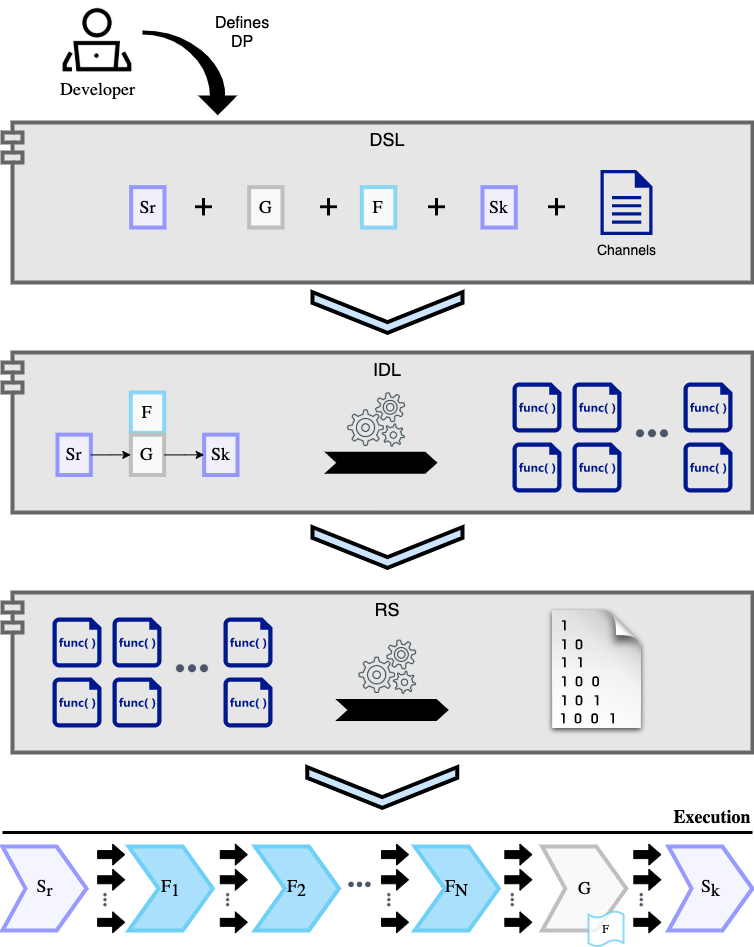
\includegraphics[width=1\textwidth, height=0.6\textheight]{dpf_haskell_v3.png}
    \caption{Architectural view of \acrshort{dpfh}}
    \label{fig:dpfh:1}
  \end{minipage}
\end{figure}

In \autoref{fig:dpfh:1} we can appreciate the different components mentioned before that are the grey boxes.

\paragraph{DSL} The user interacts with the \acrshort{dsl} component where defines how the \acrshort{dp} disposition
should be and what are the channels that are going to communicate the different stages of the pipeline: for example in the
case of \autoref{prole} that we develop the \acrshort{wcc} algorithm, the user knows that is going to received from the Input 
the edges of the graph and it needs two channels between $\iwcc$, $\gwcc$ and $\owcc$, one for sending the edges and another for sending
the accumulated connected components. 

\paragraph{IDL} The user interacts with the \acrshort{idl} which guide him to build the functions with the algorithms needed for each stage: 
$\iwcc$, $\gwcc$, $\owcc$, $\fwcc$ and actors. Based on the definition provided in the \acrshort{dsl}, the framework will indicate the user 
how that definition is interpreted in the context of \acrshort{dp} and what functions should provide.

\paragraph{RS} Once we have the \acrshort{dp} definition and the functions provided by the user with the algorithm solution, the framework
can be fed with this components to execute the program. 

\section{Implementation}
In this section we are going to describe the details of all the techniques used for implementing each of the components described before.
As we have explained in \autoref{sec:contrib}, this library it is published on Hackage~\cite{dynamic-pipeline} and the source code is open 
and can be found on this Github Repository~\cite{dynamic-pipeline-git}.

\subsection{DSL Grammar}\label{sub:sec:dsl-gram}
In order to provide a Type-safe verification in compilation time we have defined a Context Free Grammar that generates a \acrshort{dp} \acrshort{dsl} language  
and it is encoded in custom types. This allows the user to define a type-level \acrshort{dp} of the pipeline he wants to build. 
In order to do that we have the following Context Free Grammar definition.

\begin{definition}[DSL Grammar]
Lets have the grammar $\gdsl = (N, \Sigma, DB, P)$, where $N$ is the set of non-terminal symbols, $\Sigma$ the set of terminal symbols,
$DP$ is the start symbol and $P$ the generation rules, such that:

\begin{equation*}
    \boxed{
      \begin{aligned}
    N &= \{DP,S_r,S_k,G,F_b,CH,CH_s\},\\
    \Sigma &= \{\text{\mintinline{haskell}{Source}},\text{\mintinline{haskell}{Generator}},\text{\mintinline{haskell}{Sink}},\text{\mintinline{haskell}{FeedbackChannel}},\text{\mintinline{haskell}{Type}},\text{\mintinline{haskell}{Eof}},\text{\mintinline{haskell}{:=>}},\text{\mintinline{haskell}{:<+>}}\},
    \end{aligned}
    }
\end{equation*}

\begin{equation*}
  \boxed{
    \begin{aligned}
  P = \{\\
  DP  &\rightarrow S_r\ \text{\mintinline{haskell}{:=>}}\ G\ \text{\mintinline{haskell}{:=>}}\ S_k\ |\ S_r\ \text{\mintinline{haskell}{:=>}}\ G\ \text{\mintinline{haskell}{:=>}}\ F_b\ \text{\mintinline{haskell}{:=>}}\ S_k,\\
  S_r &\rightarrow \text{\mintinline{haskell}{Source}}\ CH_s,\\
  G   &\rightarrow \text{\mintinline{haskell}{Generator}}\ CH_s,\\
  S_k &\rightarrow \text{\mintinline{haskell}{Sink}},\\
  F_b &\rightarrow \text{\mintinline{haskell}{FeedbackChannel}} CH,\\
  CH_s &\rightarrow \text{\mintinline{haskell}{Channel}}\ CH,\\
  CH &\rightarrow \text{\mintinline{haskell}{Type :<+>}}\ CH\ |\ \text{\mintinline{haskell}{Eof}}\}
\end{aligned}
}
\end{equation*}
\end{definition}

In order to encode this on the language we need to generate encoded it in a Phantom type~\cite{type-index} 
to index the information that we dont want to lose and it is needed for generate the \acrshort{dp}. 
In that sense we create a Phantom type for each element of $\Sigma$.

\begin{listing}[H]
  \begin{minted}[fontsize=\small,numbers=left,frame=lines,framerule=2pt,framesep=2mm,baselinestretch=1.2,highlightlines={3,4}]{haskell}

data Source (a :: Type)
data Generator (a :: Type)
data Sink
data Eof
data Channel (a :: Type)
data FeedbackChannel (a :: Type)

  \end{minted}
  \caption{$\Sigma$ enconding of $G_{dsl}$}
  \label{src:dpfh:1}
\end{listing}
  
As we can see in \autoref{src:dpfh:1}, highlighted types are terminal symbols of $\gdsl$ that are not indexed with any Phantom type. 
This is because they do not carry any extra type information that we need to keep. In the case of \mintinline{haskell}{Sink} it is the last stage
that does not connect further with any other stage, therefore we do not need to indicate channel information. \mintinline{haskell}{Eof} it is just 
a terminal type to disambiguate the \mintinline{haskell}{Channel (a :: Type)} subtree of the full parser tree. Since \mintinline{haskell}{Channel} can carry any type, 
because we need to allow different number of channels and channels types, we need a symbol that marks end of the channel list, i.e. a sum type 
type-level encoded.

There are two more important $\Sigma$ that needs to be addressed independently which are \mintinline{haskell}{:=>} and \mintinline{haskell}{:<+>}.

\begin{listing}[H]
  \begin{minted}[fontsize=\small,numbers=left,frame=lines,framerule=2pt,framesep=2mm,baselinestretch=1.2,highlightlines={1,5}]{haskell}

data chann1 :<+> chann2 = chann1 :<+> chann2
  deriving (Typeable, Eq, Show, Functor, Traversable, Foldable, Bounded)
infixr 5 :<+>
   
data a :=> b = a :=> b
  deriving (Typeable, Eq, Show, Functor, Traversable, Foldable, Bounded)
infixr 5 :=>
   
  \end{minted}
  \caption{$\Sigma$ enconding of $G_{dsl}$ - Especial non-terminals}
  \label{src:dpfh:2}
\end{listing}

In \autoref{src:dpfh:2}, \mintinline{haskell}{:=>} and \mintinline{haskell}{:<+>} can combine 2 types. This types are syntactic sugar and different
because as we are going to see in \acrshort{idl} implementation we need two distinguishable symbols to separate the encoding of the pipeline stage ($\iwcc$, $\gwcc$, $\owcc$)
from the encoding of channel composition in the same stage, as we can appreciate in the $\gdsl$ definition.

As an user and having this few type setup we can start defining our pipelines.  
For example if we want to generate a language for \acrshort{dp} that eliminates duplicated in a stream, we know that
only need one channel connecting the stages that carries the type, in this case \mintinline{haskell}{Int}.

\begin{listing}[H]
  \begin{minted}[fontsize=\small,numbers=left,frame=lines,framerule=2pt,framesep=2mm,baselinestretch=1.2,highlightlines={}]{haskell}

type DPExample = Source (Channel (Int :<+> Eof)) 
              :=> Generator (Channel (Int :<+> Eof)) 
              :=> Sink
   
  \end{minted}
  \caption{Example of \acrshort{dp} encoded in $G_{dsl}$}
  \label{src:dpfh:3}
\end{listing}

\subsection{DSL Validation}\label{sub:sec:dsl-val}
The language generated by the grammar needs to be validate in order to avoid the user make mistake and provide an incorrect \acrshort{dp} definition.
Fortunately \acrshort{hs} provides several Type-level techniques~\cite{type-haskell} which allows us to verify properties of our programs in the language before running it, 
saving the users to write bugs and reduce errors. This verification done by the compiler is sophisticated but powerful, establishing a Curry-Howard Isomorphism~\cite{curryhoward}: 
\emph{Propositions as Types - Programs as Proof}. 

Although the language provides a lot of tools to build a type correspondence with propositional logic that can be check at compilation type, it is also known that all these
techniques requires the addition of Language Extensions that serve for that purpose. We cannot forget that even though \acrshort{hs} has more than 20 years of 
Academic Research on its core language, some of the features have been added as extensions, specially the ones that implement state of the art Type Theory concepts. 

The first thing to spot according to the definition on the previous \autoref{sub:sec:dsl-gram} is the validation of the grammar. 
In order to validate the language at type-level we use a \emph{First Class Family} with a \emph{Type-level Defunctionalization}~\cite{fun-type-function-haskell} technique.


\begin{listing}[H]
  \begin{minted}[fontsize=\small,numbers=left,frame=lines,framerule=2pt,framesep=2mm,baselinestretch=1.2,highlightlines={6,30}]{haskell}

type family And (a :: Bool) (b :: Bool) :: Bool where
    And 'True 'True = 'True
    And a b         = 'False
  

type family IsDP (dpDefinition :: k) :: Bool where
    IsDP (Source (Channel inToGen)
          :=> Generator (Channel genToOut)
          :=> Sink)
          = And (IsDP (Source (Channel inToGen))) 
                (IsDP (Generator (Channel genToOut)))
    IsDP ( Source (Channel inToGen)
           :=> Generator (Channel genToOut)
           :=> FeedbackChannel toSource 
           :=> Sink 
          )
          = And (IsDP (Source (Channel inToGen))) 
                (IsDP (Generator (Channel genToOut)))
    IsDP (Source (Channel (a :<+> more)))     
          = IsDP (Source (Channel more))
    IsDP (Source (Channel Eof))               
          = 'True
    IsDP (Generator (Channel (a :<+> more)))  
          = IsDP (Generator (Channel more))
    IsDP (Generator (Channel a))              
          = 'True
    IsDP x                                    
          = 'False
     
type family ValidDP (a :: Bool) :: Constraint where
  ValidDP 'True = ()
  ValidDP 'False = 
    TypeError
    ( 'Text "Invalid Semantic for Building DP Program"
      ':$$: 'Text "Language Grammar:"
      ':$$: 'Text "DP       -> Source CHANS :=> Generator CHANS :=> Sink"
      ':$$: 'Text "DP       -> Source CHANS :=> Generator CHANS :=> FEEDBACK 
                                            :=> Sink"
      ':$$: 'Text "CHANS    -> Channel CH"
      ':$$: 'Text "FEEDBACK -> FeedbackChannel CH"
      ':$$: 'Text "CH       -> Type :<+> CH | Eof"
      ':$$: 'Text "Example: 'Source (Channel (Int :<+> Int)) 
                            :=> Generator (Channel (Int :<+> Int)) 
                            :=> Sink'"
    )
  \end{minted}
  \caption{Validating encoded in $G_{dsl}$ - FCF}
  \label{src:dpfh:4}
\end{listing}

\acrshort{hs} Type system is fully saturated by the compiler, because otherwise it won't type checked in compilation type. 
Before of this our \mintinline{haskell}{IsValid} type as we see in \autoref{src:dpfh:4}, needs to generate the language
of the grammar providing evidence to the Type System that the user must define that language and no other is possible. 
\mintinline{haskell}{IsValid} Type Family saturates to a \mintinline{haskell}{Bool} promoted Type, not a boolean value, \mintinline{haskell}{'True} or 
\mintinline{haskell}{'False} with ticks, are promoted types not values. With this technique and defining a custom type level error defined 
in \mintinline{haskell}{ValidDP} type, the compiler will help the user to generate the correct language based on the definition.
Now we can use this types to constraint main functions and ensure the user definition will be type checked by the compiler.

\begin{listing}[H]
  \begin{minted}[fontsize=\small,numbers=left,frame=lines,framerule=2pt,framesep=2mm,baselinestretch=1.2,highlightlines={2}]{haskell}

mkDP :: forall dpDefinition filterState filterParam st.
    ( ValidDP (IsDP dpDefinition)
    , DPConstraint dpDefinition filterState st filterParam)
 => Stage (WithSource dpDefinition (DP st)) 
 -> GeneratorStage dpDefinition filterState filterParam st  
 -> Stage (WithSink dpDefinition (DP st))  
 -> DP st ()
mkDP = ...

someFunc = mkDP @DPExample ...

  \end{minted}
  \caption{Using validation of \acrshort{dp} encoded in $G_{dsl}$}
  \label{src:dpfh:5}
\end{listing}

Other details will be cover later in this chapter, but in \autoref{src:dpfh:5} we can appreciate how easy is to constraint over 
the type family defined in the Framework and compiler will show the error if the \acrshort{dp} definition is not correct.

\subsection{IDL}
\acrfull{idl} component takes the definition made on with \acrshort{dsl} grammar to interpret an generate the function definitions, 
that the user needs to fill with their algorithms for solving the specific problem definition. In \autoref{sec:dp} we have describe what are 
the behavior the user needs to provide in a \acrshort{dp} algorithm: each stage ($\iwcc$, $\gwcc$ and $\owcc$) and the $\fwcc$ with the set of Actors, 
that can be 1 or many.

The implementation of \acrshort{idl} helps the user to generate the function definitions that the user needs to complete with the implementation, 
to ensure that those functions will give a Proof of the Propositions defined on the \acrshort{dsl}, therefore the Curry-Howard Correspondence is completed~\cite{curryhoward}.

Similar techniques that we used on \autoref{sub:sec:dsl-val} is also use here. On the first hand we again use type level \emph{Defunctionalization} to 
let the compiler generates the signatures of the required functions and then Term level \emph{Defunctionalization} to interpret that functions.
At the same time some Type Index and Heterogenous List~\cite{type-index} as also used to keep track of the dynamic number and parameters types of each 
function. 

\begin{listing}[H]
  \begin{minted}[fontsize=\small,numbers=left,frame=lines,framerule=2pt,framesep=2mm,baselinestretch=1.2,highlightlines={3,4}]{haskell}

withSource :: forall (dpDefinition :: Type) st. 
              WithSource dpDefinition (DP st) 
            -> Stage (WithSource dpDefinition (DP st))
withSource = mkStage' @(WithSource dpDefinition (DP st))

withGenerator :: forall (dpDefinition :: Type) (filter :: Type) st. 
                 WithGenerator dpDefinition filter (DP st) 
              -> Stage (WithGenerator dpDefinition filter (DP st))
withGenerator = mkStage' @(WithGenerator dpDefinition filter (DP st))

withSink :: forall (dpDefinition :: Type) st. 
            WithSink dpDefinition (DP st) 
           -> Stage (WithSink dpDefinition (DP st))
withSink = mkStage' @(WithSink dpDefinition (DP st))


  \end{minted}
  \caption{Using withXXXX Interpreters of \acrshort{dp} encoded in $G_{dsl}$}
  \label{src:dpfh:6}
\end{listing}

As we can see on \autoref{src:dpfh:6} there is \mintinline{haskell}{Stage *} class type that we use for 
the Defunctionalization at term level, and that class is polymorphic in the type of Stage it can build.
The differents \mintinline{haskell}{WithSource}, \mintinline{haskell}{WithGenerator} and \mintinline{haskell}{WithSink}
\emph{Associate Type Families} help the compiler to deduce the signature of the function that the user should provide for that Stage.


\begin{listing}[H]
  \begin{minted}[fontsize=\small,numbers=left,frame=lines,framerule=2pt,framesep=2mm,baselinestretch=1.2,highlightlines={12,16}]{haskell}

type family WithSource (dpDefinition :: Type) (monadicAction :: Type -> Type) :: Type where
  WithSource (Source (Channel inToGen) 
                :=> Generator (Channel genToOut) 
                :=> Sink) monadicAction
        = WithSource (ChanIn inToGen) monadicAction
  WithSource (Source (Channel inToGen) 
                :=> Generator (Channel genToOut) 
                :=> FeedbackChannel toSource 
                :=> Sink) monadicAction
        = WithSource (ChanOutIn toSource inToGen) monadicAction
  WithSource (ChanIn (dpDefinition :<+> more)) monadicAction         
        = WriteChannel dpDefinition -> WithSource (ChanIn more) monadicAction
  WithSource (ChanIn Eof) monadicAction                              
        = monadicAction ()
  WithSource (ChanOutIn (dpDefinition :<+> more) ins) monadicAction  
        = ReadChannel dpDefinition -> WithSource (ChanOutIn more ins) monadicAction
  WithSource (ChanOutIn Eof ins) monadicAction                       
        = WithSource (ChanIn ins) monadicAction
  WithSource dpDefinition _                                          
        = TypeError
          ( 'Text "Invalid Semantic for Source Stage"
            ':$$: 'Text "in the DP Definition '"
            ':<>: 'ShowType dpDefinition
            ':<>: 'Text "'"
            ':$$: 'Text "Language Grammar:"
            ':$$: 'Text "DP       -> Source CHANS 
                                      :=> Generator CHANS 
                                      :=> Sink"
            ':$$: 'Text "DP       -> Source CHANS 
                                      :=> Generator CHANS 
                                      :=> FEEDBACK :=> Sink"
            ':$$: 'Text "CHANS    -> Channel CH"
            ':$$: 'Text "FEEDBACK -> FeedbackChannel CH"
            ':$$: 'Text "CH       -> Type :<+> CH | Eof"
            ':$$: 'Text "Example: 'Source (Channel (Int :<+> Int)) 
                                    :=> Generator (Channel (Int :<+> Int)) 
                                    :=> Sink'"
          )
  \end{minted}
  \caption{WithSource Associate Type Details}
  \label{src:dpfh:7}
\end{listing}

In \autoref{src:dpfh:7} we can see in the highlighted lines how the type induction is 
expanding a function definition of the form \mintinline{haskell}{a -> b -> ...} depending on 
\acrshort{dp} language definition. Lets see how \mintinline{haskell}{Stage} was defined in order 
to read saturate this type and ask the user the proper function according to that generated type.

\begin{listing}[H]
  \begin{minted}[fontsize=\small,numbers=left,frame=lines,framerule=2pt,framesep=2mm,baselinestretch=1.2,highlightlines={12,16}]{haskell}

data Stage a where
  Stage :: Proxy a -> a -> Stage a

mkStage' :: forall a. a -> Stage a
mkStage' = Stage (Proxy @a)
    
  \end{minted}
  \caption{Stage Data Type}
  \label{src:dpfh:8}
\end{listing}

It is use a simple \mintinline{haskell}{Proxy a} phantom type technique to remember the type definition generated by \mintinline{haskell}{a}.
In the case of \mintinline{haskell}{withSource} interpreter shown in \autoref{src:dpfh:6}, $\mintinline{haskell}{a} \thicksim \mintinline{haskell}{WithSource definition}$, therefore 
when compiler fully saturates the type it can tell the user what is the function that \mintinline{haskell}{Stage} should contain.

\subsection{Generator and Filter}

\subsection{RS - Runtime System}

\section{Libraries and Tools}

\section{Chapter Summary}

